\section{Architecture}
\label{sec:architecture}

This section will describe two different architecture models that can be used to serve content to users over the Internet. The two architectures that will be described are the Client-server model and the Peer-to-Peer model.

\subsection{Client-Server Model}
The Client-Server model is the model most often used to serve web pages and generally access the Internet. The model consists of two parts, a client and a server.
The basic structure of the client-server model can be seen in \autoref{fig:client-server}.

\begin{figure}[ht]
  \centering
    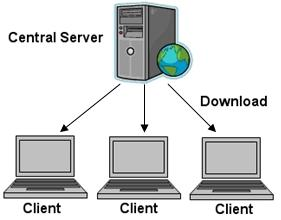
\includegraphics[width=0.5\textwidth]{img/client_server.jpg}
  \caption{Client-Server Technology \citep{ClientServer}}
  \label{fig:client-server}
\end{figure}

The client runs on a users computer, and is responsible for downloading information and if needed rendering it as web pages, graphics etc. For web pages, this rendering is usually done in a browser, but the model does not change with different types of data.
The server is a computer which is connectible through either a local network or the Internet. When a client computer connects to a server, the server will serve the content that has been requested by the client. For web pages this is usually some form of HTML files and scripts, but a server can also just serve a single file for download.

The Client-Server model is used in almost all programs. Applications often use the Client-Server model to stay updated, and video games often use the model to connect multiple clients to each other such that they can play with or against each other in a multiplayer environment.

The Client-Server model requires more bandwidth and more servers as more users is accessing them. This is because the owners of the servers must be able to serve their content to every user trying to access it. Otherwise a user will experience a degraded quality of service or may not be able to access the content at all.

\subsection{Peer-to-Peer}
An alternative to the Client-Server model is the Peer-to-Peer model.
The Peer-to-Peer model is like the Client-Server model without the server.
Instead all the clients connect to each other in a decentralized system, as seen in \autoref{fig:p2p}.

\begin{figure}[ht]
  \centering
    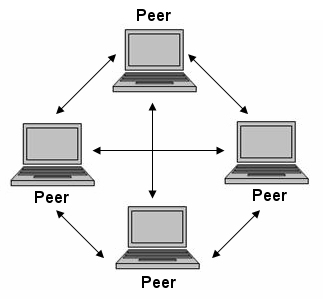
\includegraphics[width=0.4\textwidth]{img/p2p.jpg}
  \caption{Peer-to-Peer Technology \citep{PeerToPeer}}
  \label{fig:p2p}
\end{figure}

One of the positive aspects of this model is, that it drastically reduces the cost that a Client-Server based system has to keep servers running by avoiding the server completely.
However, the Peer-to-Peer model also has some negative aspects.
One of the negative aspects is that most of the peers in a Peer-to-Peer network consist of home PC's on home network connections. This means that they may not always be available, and thus if no or few people are have the content available it becomes difficult to access at all.

This model is often only used for specialized tasks, such as file sharing between users or downloading large amounts of data that a company does not want to pay to host.
The Peer-to-Peer model will in most cases require specialized software to be used.